\documentclass[twocolumn,12pt]{article}
\usepackage[utf8]{inputenc}
\usepackage{lmodern} %fuente a utilizar
\usepackage{setspace}
\usepackage{geometry}
\usepackage{fancyhdr}
\usepackage{graphicx} % Paquete para manejar imágenes
\usepackage[absolute,overlay]{textpos} % Para posicionar la imagen
\usepackage{datetime2} % Para personalizar el formato de la fecha
\usepackage{amsmath}
\usepackage{amssymb}
\usepackage{graphicx}
\usepackage{multicol}
\geometry{
    a4paper,
    left=18mm,
    right=18mm,
    top=32mm, % Ajusta el margen superior si es necesario
    bottom=20mm,
    headsep=35mm, % Ajusta el espacio entre encabezado y texto
}


% Configuración de espaciado entre líneas
\setstretch{1.5}

% Define the header
\pagestyle{fancy}
\fancyhf{} % Clear all header and footer fields
\fancyhead[L]{
\vspace{-0.5cm}

\includegraphics[width=5cm]{Multimedia/logo_uai.png}} % Adjust the width as needed
\renewcommand{\headrulewidth}{0.5pt} % Line thickness for the header separator
\fancyfoot[C]{\thepage}

\begin{document}
	
	\begin{titlepage}
		\centering
                % Adjust vertical space to move the content higher
            \vspace*{-0.5in} % Reduced to move everything up
		\vspace*{1in}
		
		% Configuración de la imagen en la esquina superior derecha
		\begin{textblock*}{0in}(12.5cm,2cm) % (ancho del bloque, coordenada-x, coordenada-y)
			
\includegraphics[width=3in,height=3in,keepaspectratio]{./Multimedia/logo_uai.png}
		\end{textblock*}
		
		% Línea horizontal sobre el título
		\noindent\rule{1\textwidth}{0.4pt}
		\begin{flushleft}
			\textbf{FIS101}
		\end{flushleft}
		
		\vspace{0in} % Espacio entre la línea y el título
		
		% Título del Informe
		\begin{flushleft}
			\huge
			\textbf{Laboratorio 1\\}
			\large
			\textbf{Medición de la aceleración en caída libre:\\ aplicando el principio de Galileo}
			\vspace{0.4in} % Espacio entre el título y la línea inferior
		\end{flushleft}
		
		% Línea horizontal debajo del título
		\noindent\rule{1\textwidth}{0.4pt}
		
		\vspace{0.8in}
		
		% Información del informe
		\large
		\begin{flushleft}
			\textbf{Integrantes:}
			
			\begin{itemize}
				\item Ferré Díaz Felipe
				\item Muñoz Escobedo Benjamin 
                \item Quezada Escobar Víctor
			\end{itemize}
			
			\vspace{0.2in}
			
			\large
			\textbf{Curso:} Física I; Sección 1
			
			\vspace{0.2in}
			
			\large
			\textbf{Profesor:} David Aguayo Vera
		\end{flushleft}
		
		\vspace{0.2in}
		
		\begin{flushright}
			\Large
			Fecha: \today % Fecha actual en formato de año
		\end{flushright}
		
		
		
		\vspace{1in}
	\end{titlepage}
	
	% Secciones del documento
	\section{Resumen}
 El objetivo de este Laboratorio fue medir la aceleración de un carro en diferentes ángulos del plano, comparando los resultados obtenidos con herramientas tecnológicas actuales. Se determinó que la componente de aceleración en nuestro eje referencial inclinado aumenta conforme se incrementa la inclinación. Los resultados experimentales fueron consistentes con los valores teóricos dentro de las consideraciones esperadas que implicaban el desprecio de la resistencia del medio en el que se realizó el experimento.
	
	\section{Introducción}
En este experimento se replicó de manera satisfactoria los experimentos en que Galileo Galilei comprobó su hipótesis de que un objeto en caída libre adquiriría cantidades iguales de velocidad en tiempos iguales utilizando un plano inclinado. Para lo anterior, Galileo diseñó un experimento que consistía en una rampa donde deslizaría distintos pesos en distintos grados para comprobar que la tasa de aceleración no dependía de las masas utilizadas. Contrastaremos los datos obtenidos experimentalmente con el marco teórico obtenido en las cátedras de Física I, principalmente con las ecuaciones itinerarios en los ejes "X" e "Y" referenciales, y el cálculo de su componente resultante según la suma trigonométrica de los vectores obtenidos.
		
	\section{Ecuaciones}
 	A continuación presentamos las ecuaciones base utilizadas para los cálculos realizados en el marco teórico del experimento propuesto. De las ecuaciones itinerario en los ejes referenciales X e Y obtendremos las ecuaciones de aceleración y velocidad. En conjunto con las ecuaciones de transformación de coordenadas cartesianas a polares, obtendremos los valores teóricos de aceleración en distintos ángulos de lanzamiento de nuestro carro a través de la rampa.
 	\vspace{-1cm}
 	\begin{center}

 	\begin{equation}
 		\centering
 		x_{(t)} = y_{0} + V_{0} \cdot t + a \cdot t^{2} 
 		\tag*{(1)} % ecuación itinerario eje x
 	\end{equation}
 		
 	\vspace{-0.8cm}
 	
 	\begin{equation}
 		\centering
 		y_{(t)} = y_{0} + V_{0} \cdot t + a \cdot t^{2} \tag*{(2)} % ecuación itinerario eje y
 	\end{equation}
 	
 	\vspace{-0.8cm}  
 	
	\centering\text{Ec. itinerarios relativa a los ejes x e y.}
	
	\begin{equation}
		\centering
		x = r \cdot Cos (\Theta) \tag*{(3)} 
	\end{equation}
	
	\vspace{-0.4cm}
	
	\begin{equation}
		\centering
		y = r \cdot Sen (\Theta) \tag*{(4)} 
	\end{equation}
	
	\vspace{-0.4cm}  
	
	\centering\text{Ec. conversión de coordenadas}
	\centering\text{polares a cartesianas.}
	
	\begin{equation}
	\centering
	r = \sqrt{x^{2} + y^{2}} \tag*{(5)} 
	\end{equation}
	\vspace{-0.4cm}
	\begin{equation}
	\centering
	\Theta = tan^{-1} \cdot \left( \frac{y}{x} \right) \tag*{(6)} 
	\end{equation}
	\vspace{-0.4cm}  
	\centering\text{Ec. conversión de coordenadas}
	\centering\text{cartesianas a polares.}
	\end{center}
	
	\vspace{1cm}
	\begin{justify}
	De las ecuaciones anteriores, podemos obtener, considerando el riel como referencia para nuestro eje x, y el eje y perpendicular al riel, las siguientes ecuaciones que nos permitirán calcular las aceleraciones, velocidades y ecuaciones itinerario resultantes y compararlas con los datos obtenidos en el ejercicio experimental basados en la aceleración obtenida por el instrumento PocketLab (valor promedio medido: 9,82 m/s^{2}).
    \end{justify}
	\vspace{-1cm}
	\begin{center}
	\begin{equation}
	\centering
	a_{x} = g \cdot Sen (\Theta) \tag*{(7)} 
	\end{equation}
	
	\vspace{-0.4cm}  
	
	\centering\text{Ec. aceleración en el eje x.}
	\end{center}
	
	Debido a que estamos en un plano inclinado, tomado como ejes referenciales, se presenta la ecuación 7, con a como aceleración en el eje x, g como gravedad medida por los instrumentos de laboratorio y $\Theta$ el ángulo del riel con respecto a la mesa horizontal donde está ubicada.
	\vspace{-0.5cm}
	\begin{center}
	\begin{equation}
	\centering
	v_{x(t)} = v_{0} + a_{x}\cdot t \tag*{(9)} 
	\end{equation}
	
	\vspace{-0.4cm}  
	
	\centering\text{Ec. velocidad vs tiempo a lo largo del eje x.}
	
		\begin{equation}
	\centering
	x_{(t)} = x_{0} + v_{0} \cdot t + \left( \frac{1}{2} \right) \cdot a_{x}\cdot t^{2} \tag*{(10)} 
	\end{equation}
	
	\vspace{-0.4cm}  
	
	\centering\text{Ec. posicion vs tiempo a lo largo del eje x.}
	\end{center}

        Deducimos de las a fórmulas itinerario la formula para calcular la velocidad final, tomando datos teóricos y prácticos descritos a continuación:
        \vspace{0.8cm} 
	\begin{equation}
        \centering
	v_f = \sqrt{v_i^2 + 2 \cdot a \cdot x}\tag{11}
	\end{equation}
 	\vspace{-0.4cm} 
	Donde:
	\begin{itemize}
		\item \(v_f\) es la velocidad final en el punto B (en metros por segundo, m/s).
		\item \(v_i\) es la velocidad inicial en el punto A (valor práctico obtenido de las grabaciones, en metros por segundo, m/s).
		\item \(a\) es la aceleración a lo largo del plano inclinado (valor calculado en base a las lecturas del acelerómetro y el cálculo de las componentes de x e y de la gravedad en metros por segundo al cuadrado, m/s²).
		\item \(x\) es el desplazamiento a lo largo del plano inclinado desde el punto A hasta el punto B (en metros, m).
	\end{itemize}
	
	\section{Metodología}
	El experimento consistió en posicionar un carro y deslizarlo sobre un plano inclinado. Utilizamos la cámara de nuestros celulares para grabar la caída y procesar el video en el software propuesto por el profesor y obtener los graficos de posición y velocidad para diferentes ángulos del riel en referencia sobre el plano horizontal. Los materiales utilizados para el experimento fueron los siguientes:
	
	\begin{enumerate}
	\item Riel Pasco.
	\item Carro de colisiones Pasco.
	\item Indicador de ángulo Pasco.
	\item Masa adicional.
	\item Balanza digital.
	\item Acelerómetro PocketLab.
	\item Teléfono celular para grabar vídeo.
	\item Computador con el software Tracker. 
	\item Regla metálica.
	\end{enumerate}	
	
	\begin{figure}[h]
	\centering
	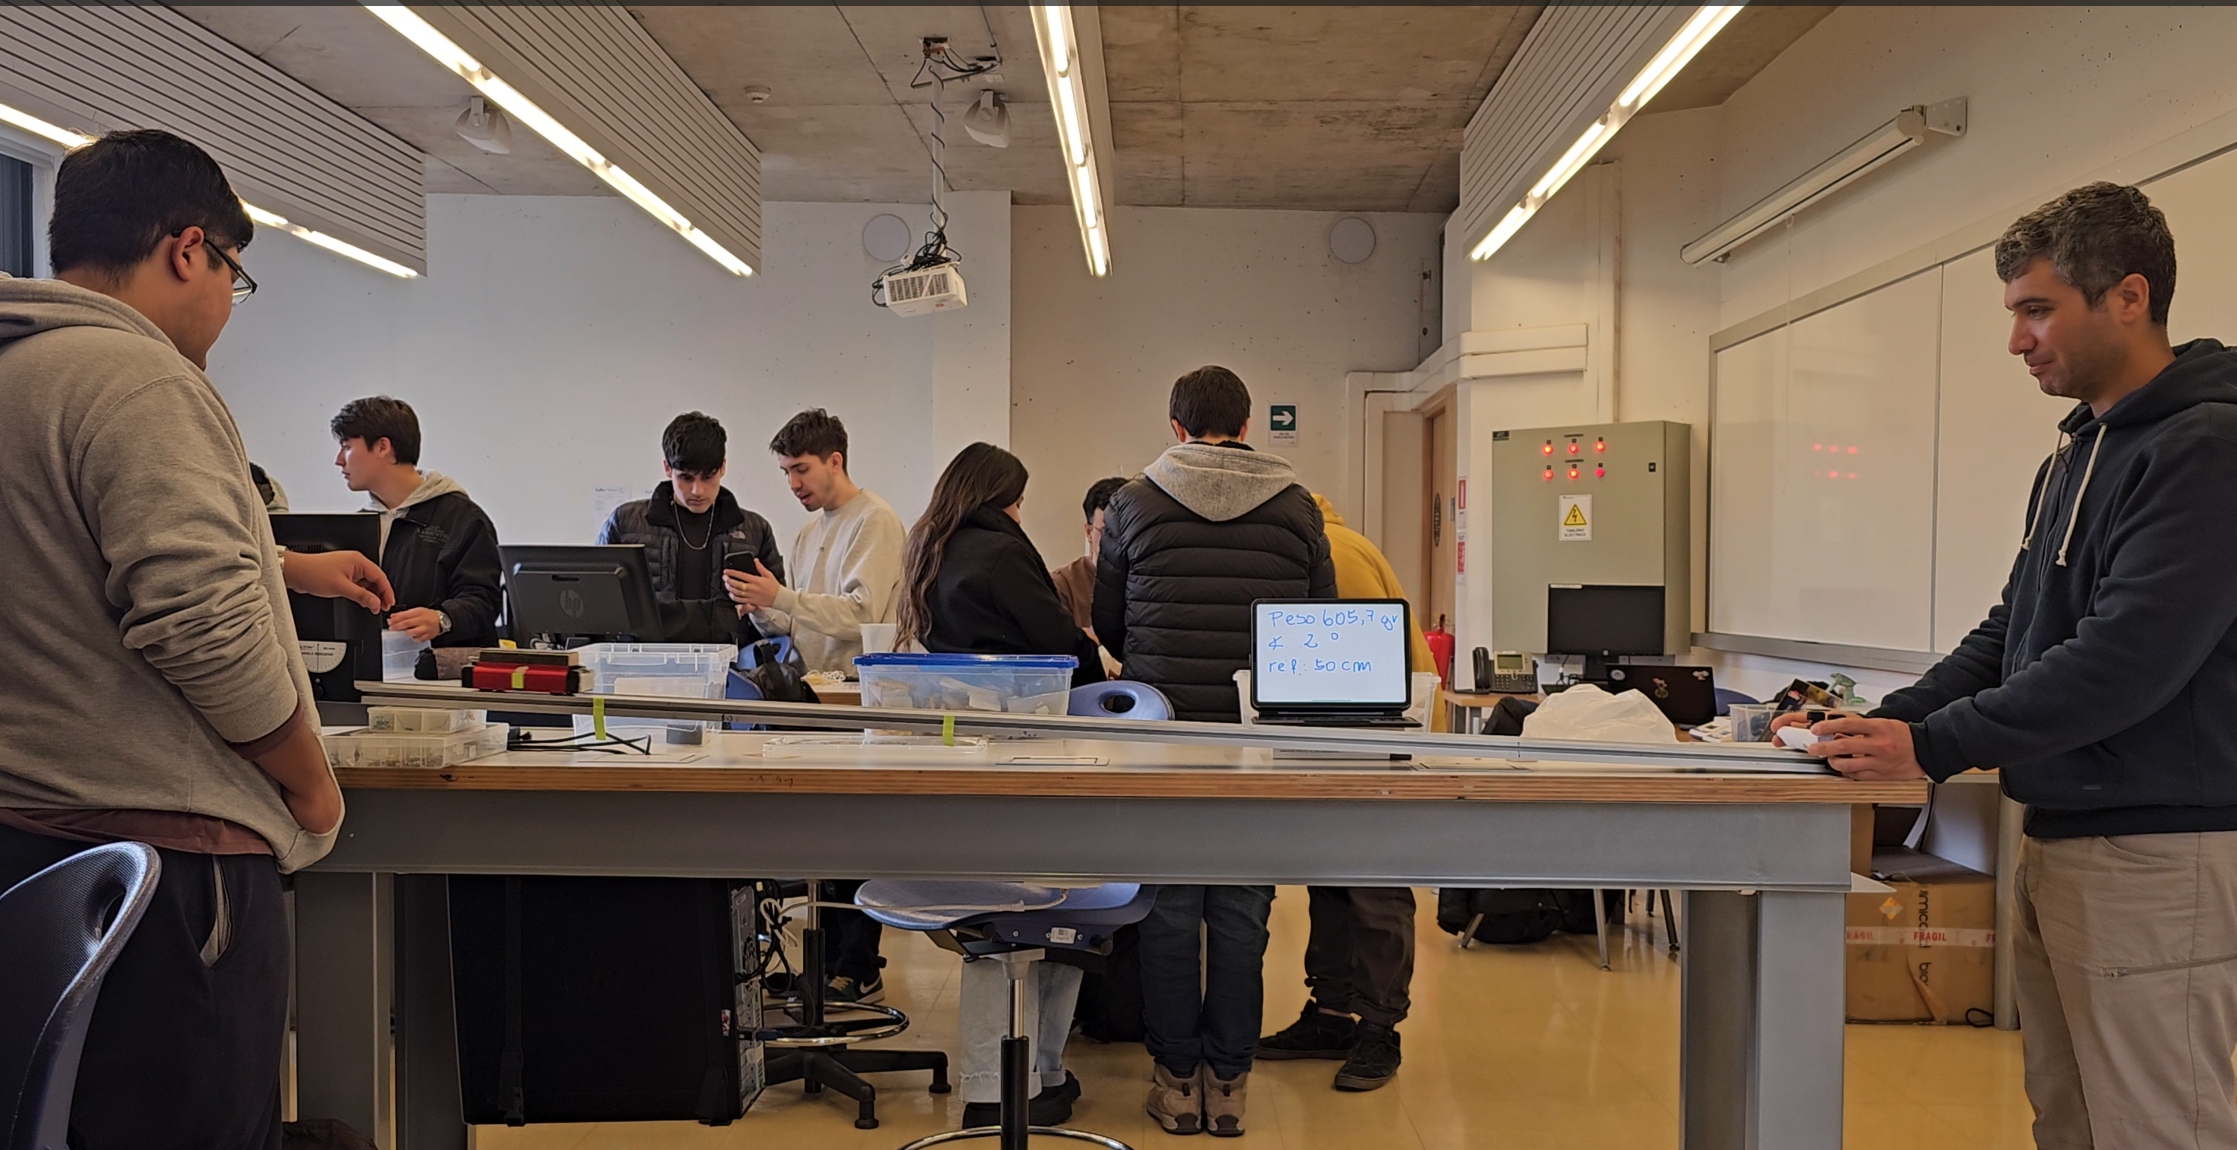
\includegraphics[width=0.5\textwidth]{./Multimedia/fotografia_laboratorio.png}
	\caption{ Procedimiento experimental}
	\label{Imagen:mi_imagen}
	\end{figure}

        El equipo de trabajo realizó 3 mediciones por cada ángulo de caída escogido, los cuales fueron 2, 4, 8, 10 y 14 grados, con la masa propia del carro Pasco y una masa adicional. El carro fue arrojado desde el extremo superior del riel Pasco sin imprimir una fuerza adicional en el inicio de su recorrido, se tomaron los vídeos correspondientes y se procesaron en el software Tracker. En dicho riel se realizaron dos marcas, A y B, distantes a 500 milímetros la una de la otra (Figura 2). Luego, se realizó la medición de la gravedad con el acelerómetro PocketLab para aplicar dicho valor en los cálculos de las tablas del presente documento. En la tabla 1 quedó demostrado cómo la diferencia entre la aceleración calculada para el mismo ángulo, con y sin peso, es despreciable, quedando así probado que la masa no afecta ni la velocidad ni la aceleración. Tomando como eje x referencial al riel inclinado, con la ecuación de aceleración (ecuación 7), con la ecuación itinerario (ecuación 10), y operaciones trigonométricas deducimos componente teórica de la aceleración en el eje x y calculamos la velocidad teórica que alcanzaría el carro al final del recorrido del riel (tabla 2). Luego con la aceleración teórica y una velocidad practica promedio en cada lanzamiento obtenida en el punto A (figura 2), calculamos una velocidad teórica en el punto B (figura 2) y la contrastamos con la velocidad promedio en cada lanzamiento en el punto B.  
	
	\section{Resultados}
	A continuación presentamos una serie de tablas y gráficos que expresan los resultados obtenidos teóricos-prácticos. Las aceleraciones de la tabla 1 fueron resultado de las pendientes de velocidad práctica entregadas por el software de análisis en cada lanzamiento. La tabla dos considera la aceleración teórica, la cual coincide con la práctica. Además se entrega el valor de velocidad que debería tener el carro en un recorrido completo del riel Pasco. La tabla 3 muestra un contraste útil de valores reales y prácticos.
	
	

	\onecolumn
        \subsection{Tablas}
	\begin{table}[h!]
	\centering
	\begin{tabular}{|c|c|c|}
	\hline
	\textbf{Ángulo de inclinación} & \multicolumn{2}{c|}{\textbf{Aceleración del cuerpo [m/s\(^2\)]}} \\ \cline{2-3}
	\textbf{} & \textbf{Sin masa adicional} & \textbf{Con masa adicional} \\ \hline
	2\textdegree & 0.371 & 0.373 \\ \hline
	4\textdegree & 0.695 & 0.697 \\ \hline
	8\textdegree & 1.24 & 1.26 \\ \hline
	10\textdegree & 1.68 & 1.69 \\ \hline
	14\textdegree & 2.37 & 2.37 \\ \hline
	\end{tabular}
	\caption{Tabla de aceleraciones experimentales en función del ángulo de inclinación.}
	\label{tabla:aceleraciones}
	\end{table}
	
	\begin{table}[h!]
	\centering
	\begin{tabular}{|c|c|c|}
	\hline
	\textbf{Ángulo de inclinación} & \textbf{Aceleración [m/s\(^2\)]} & \textbf{Velocidad final [m/s]} \\ \hline
	2\textdegree & 0.342 & 1.17 \\ \hline
	4\textdegree & 0.684 & 1.65 \\ \hline
	8\textdegree & 1.36 & 2.33 \\ \hline
	10\textdegree & 1.71 & 2.62 \\ \hline
	14\textdegree & 2.37 & 3.08 \\ \hline
	\end{tabular}
	\caption{Tabla de aceleraciones teóricas y velocidades teóricas en función del ángulo de inclinación y el largo total del riel Pasco.}
	\label{tabla:caida_galileo}
	\end{table}

        \begin{figure}[h]
            \centering
            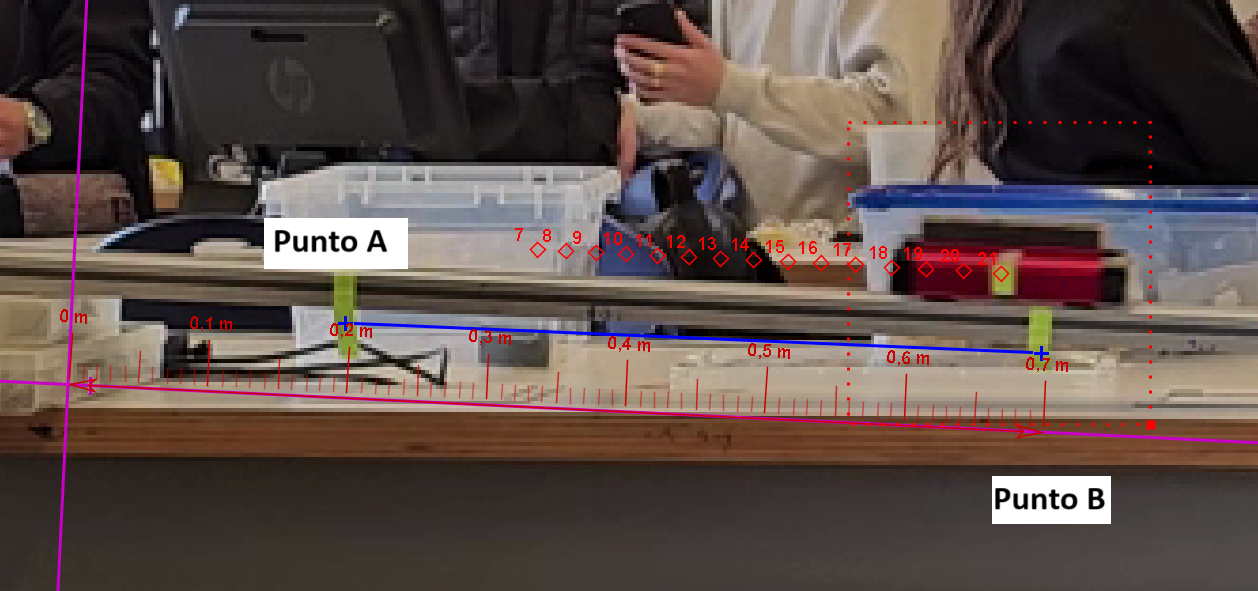
\includegraphics[width=0.6\textwidth]{Lab1/Multimedia/cond_exp.png}
            \caption{Condiciones experimentales a considerar para la interpretación de las tablas.}
            \label{fig:imagen}
        \end{figure}

        \begin{table}[h!]
		\centering

		\begin{tabular}{|c|c|c|c|c|}
			\hline
			\rowcolor{white} % Color de fondo para la primera fila
			Grados & Acel. Teo. eje x & V_{A} Pract.  & V_{B} Pract. & V_{B} Teo. \\ \hline
			2 grados & 0,342 [m/s^{2}] & 0,555 [m/s] & 0,788 [m/s] & 0,8062 [m/s] \\ \hline
			4 grados & 0,684 [m/s^{2}] & 0,747 [m/s] & 1,095 [m/s] & 1,114 [m/s] \\ \hline
			8 grados & 1,360 [m/s^{2}] & 1,004 [m/s] & 1,405 [m/s] & 1,539 [m/s] \\ \hline
			10 grados & 1,710 [m/s^{2}] & 1,126 [m/s] & 1,677 [m/s] & 1,727 [m/s] \\ \hline
			14 grados & 2,370 [m/s^{2}] & 1,349 [m/s] & 2,005 [m/s] & 2,043 [m/s] \\ \hline
		\end{tabular}
		\caption{Tabla de comparación de velocidades teóricas y prácticas en A y B.}
		\label{tabla:caida_galileo}
	\end{table}

    \onecolumn
    \subsection{Gráficos}

    Los gráficos del 1 al 5 muestran la relación entre la velocidad y el tiempo con distintos ángulos. Con el análisis de estos, podemos ver que la masa no influye en la pendiente y que los resultados se ajustan a la teoría.
    El gráfico 6 muestra la relación entre la aceleración y el ángulo, probando así los principios de Galileo.
    
    % Cambiar a una sola columna
    
    \begin{figure}[h]
        \centering
        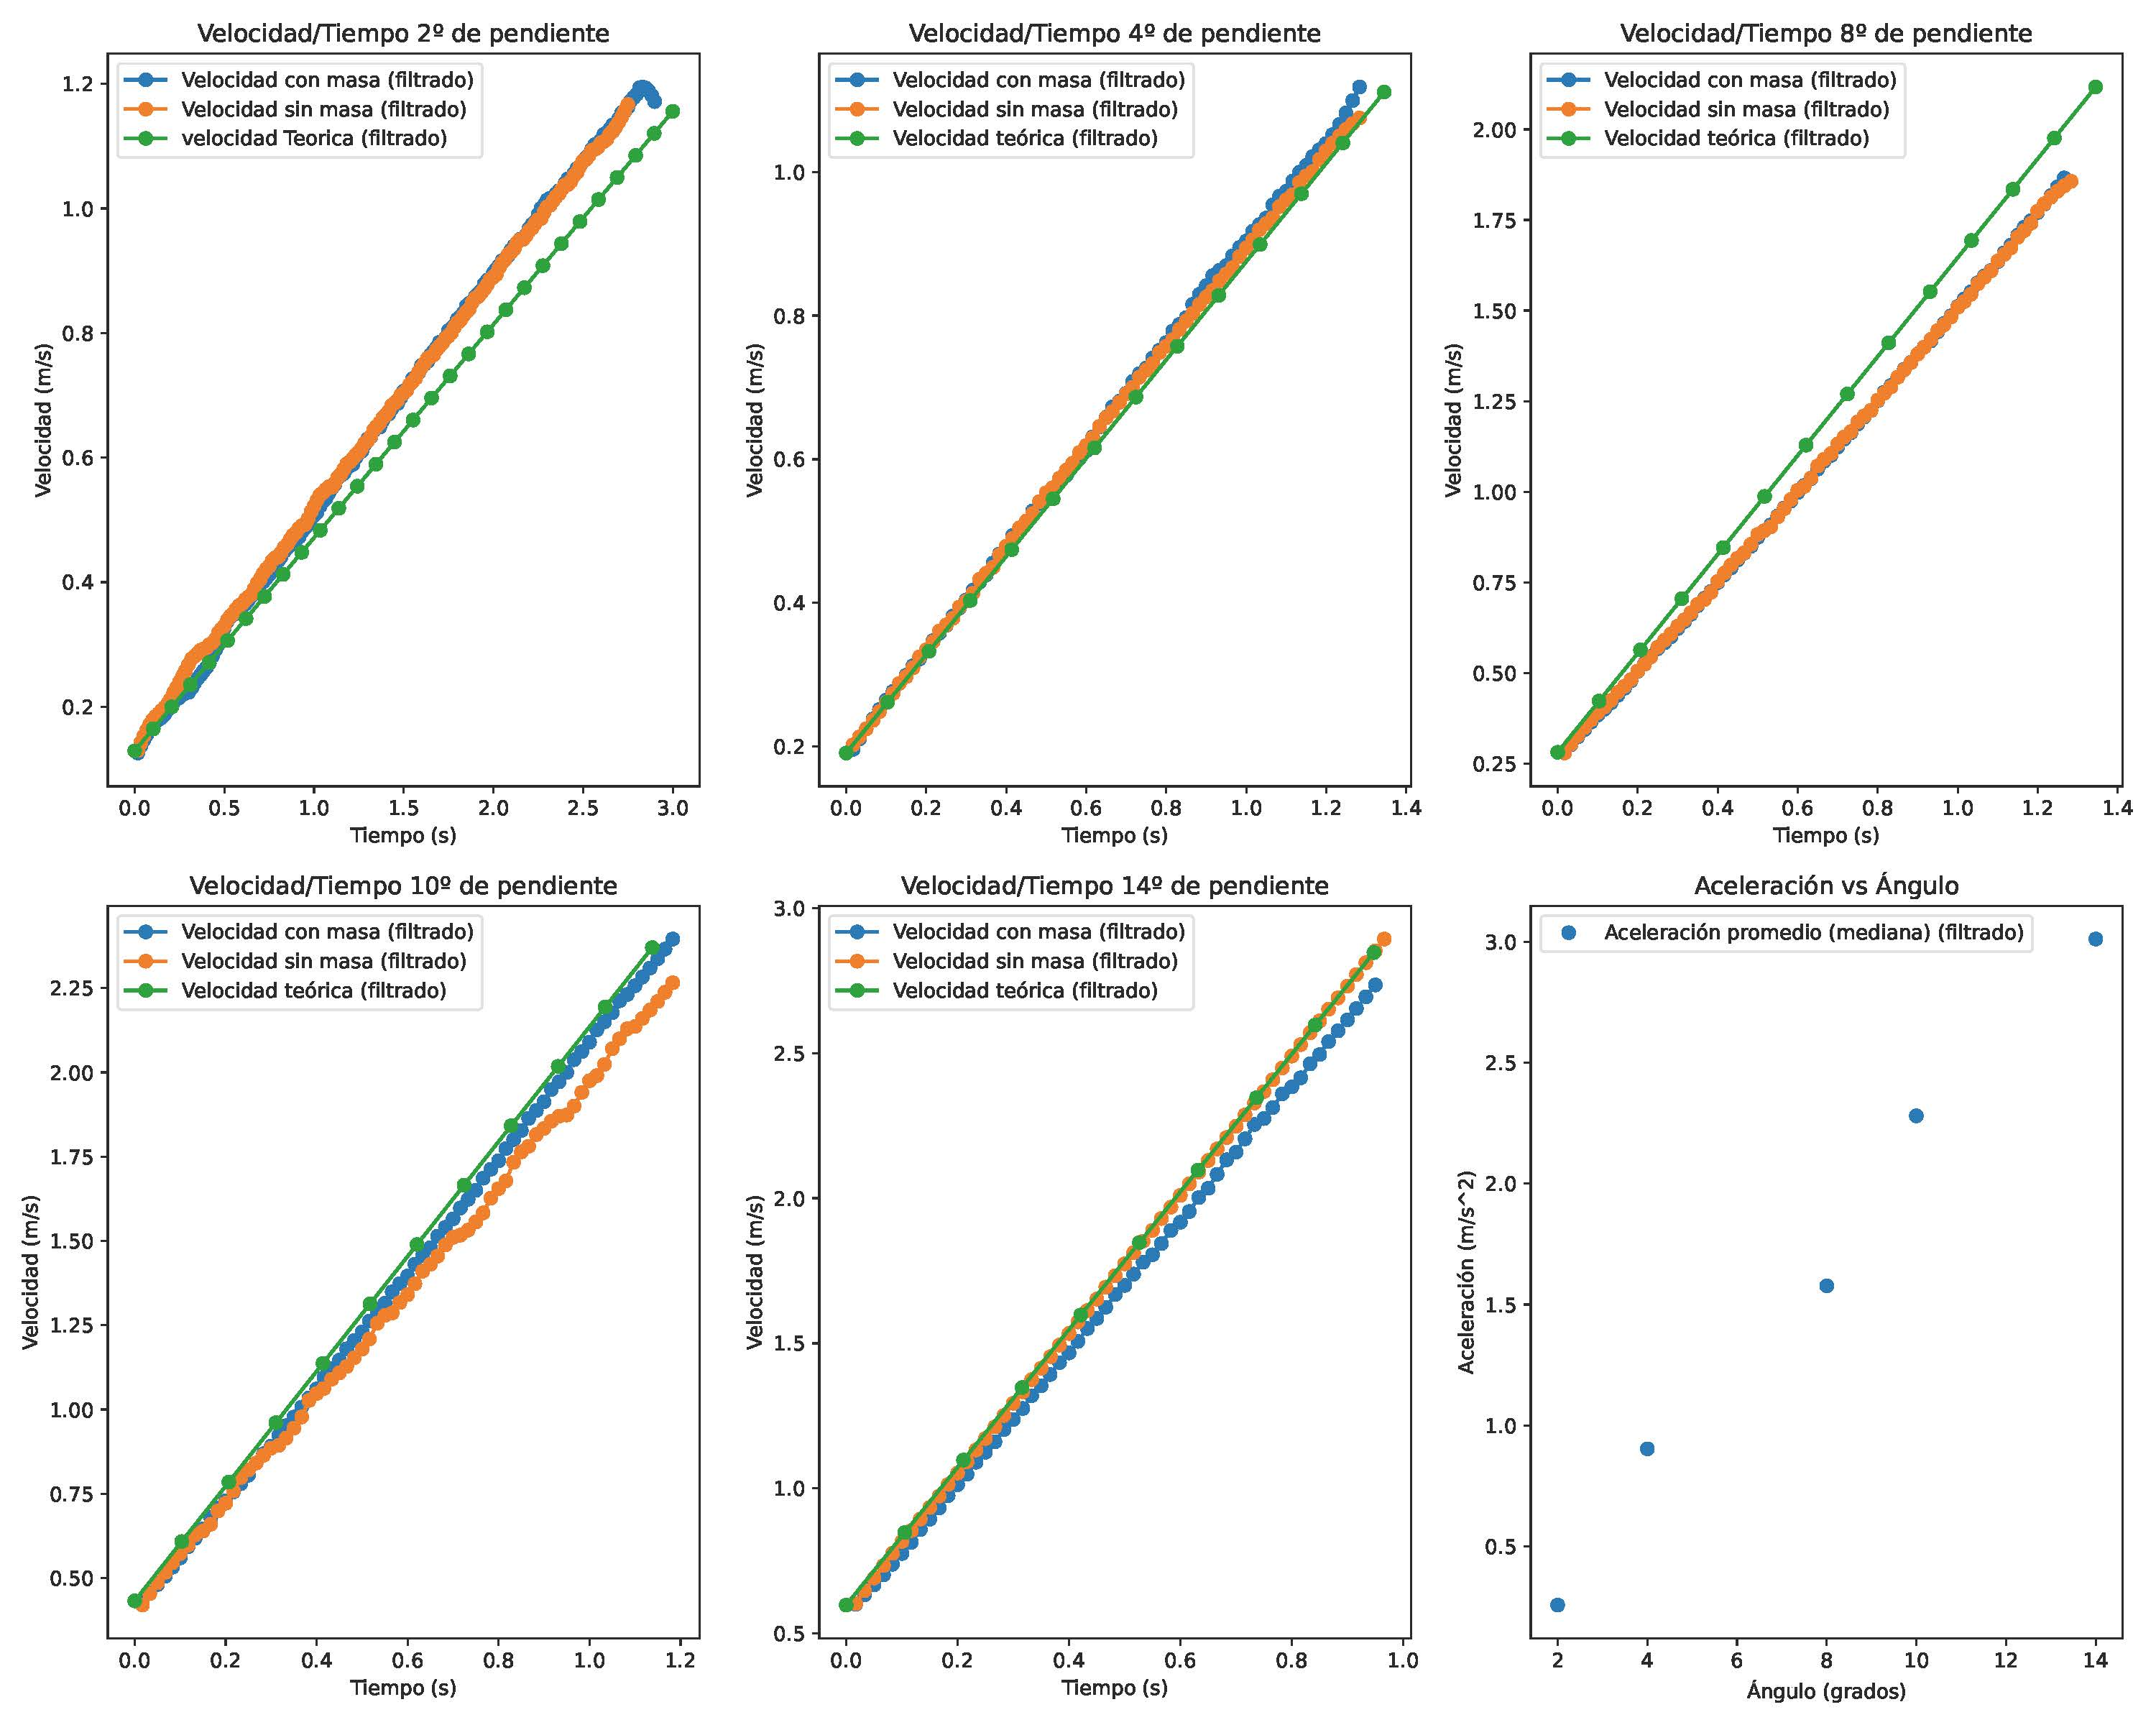
\includegraphics[width=1\textwidth]{Lab1/Multimedia/grafico1.jpg}
        \caption{Velocidad/Tiempo y aceleración/Ángulo.}
        \label{fig:imagen}
    \end{figure}

    \twocolumn
    
    \section{Resultados}
    
    El laboratorio confirmó que la aceleración es proporcional al ángulo de inclinación y que la masa no afecta la aceleración. Esto fue consistente tanto en los resultados experimentales como en los teóricos, calculados con el PocketLab.
    
    
    \subsection{Análisis de errores}
    Una de las principales fuentes de error fue el software Tracker, que se utilizó para extraer los datos de los videos. Esto se debió a que, en muchas ocasiones, los datos presentaban inconsistencias o ruido. Para contrarrestar esto, utilizamos un filtro de datos llamado Savitzky-Golay, el cual nos permitió mejorar la precisión de los datos. Como se menciono anteriormente, el contraste entre los datos prácticos y los cálculos teóricos se ve afectado al desprecio de la resistencia del medio en que fue realizado el experimento.
    
    \subsection{Comparación con la teoría}
    Los resultados fueron consistentes con los de Galileo y con la teoría sobre que la aceleración en un plano inclinado solo depende de su ángulo y no de la masa del objeto.
    
    \subsection{Conclusiones}

    El laboratorio demostró que la aceleración y la velocidad dependen del ángulo de inclinación y no de la masa del objeto móvil, validando nuestras predicciones teóricas, así como las de Galileo. Recomendamos no superar los 14 grados con el riel Pasco para evitar riesgos en el daño personal o de equipo, además de el uso de una cámara High Frame Rate para evitar el ruido en el análisis de los vídeos.
    
    \section{Referencias bibliográficas}
    \begin{itemize}
        \item Serway, R. A., & Jewett, J. W. (2014). \textit{Physics for Scientists and Engineers with Modern Physics} (9th ed.). Cengage Learning.
        \item Young, H. D., & Freedman, R. A. (2016). \textit{University Physics with Modern Physics} (14th ed.). Pearson. 
        \item Hunter, J. D. (2007). Matplotlib: A 2D Graphics Environment. \textit{Computing in Science \& Engineering}, \textit{9}(3), 90–95. https://doi.org/10.1109/MCSE.2007.55
        \item Savitzky, A., & Golay, M. J. E. (1964). Smoothing and Differentiation of Data by Simplified Least Squares Procedures. \textit{Analytical Chemistry}, \textit{36}(8), 1627–1639. https://doi.org/10.1021/ac60214a047
    \end{itemize}
    

	

\end{document}

